% $Header: https://svn.ita.chalmers.se/repos/security/edu/course/computer_security/trunk/assignment/3/template/latex/report.tex 611 2013-02-20 13:33:23Z pk@CHALMERS.SE $
%
%

\documentclass[a4paper,twoside,11pt]{article}

\usepackage{etoolbox}
\usepackage[utf8]{inputenc}
\usepackage{microtype}

\usepackage[pdftex,hidelinks]{hyperref}
\hypersetup{
    pdfstartview=FitH,
%    pdftitle={},
%    pdfauthor={},
%    pdfsubject={},
%    pdfkeywords={}
%    bookmarks,
%    bookmarksopen,
%    colorlinks,
%    linkcolor=blue,
%    citecolor=blue,
%    urlcolor=magenta,
}
\usepackage[english]{babel}
\usepackage[T1]{fontenc}
\usepackage{geometry}
\usepackage{fancyhdr}


% Setup bibliography
\usepackage{csquotes}
\usepackage[backend=biber, natbib=true, maxnames=2, minnames=1, 
maxbibnames=10, minbibnames=6, citestyle=numeric-comp, sorting=none, 
firstinits=true]{biblatex}
%\providecommand{\bibfont}{\footnotesize}
%\renewcommand{\bibfont}{\footnotesize}

% To be used for colors
\usepackage{color}
\usepackage[usenames,dvipsnames,svgnames,table]{xcolor}

% Useful Packages
\usepackage{amsmath}
\usepackage{amsthm}
\usepackage{amsfonts}

\usepackage{breakurl}
\usepackage{paralist}
\usepackage{graphicx}
\usepackage{epsfig}
\usepackage{tabularx}
\usepackage{subfigure}
\usepackage[symbol]{footmisc}


\usepackage{listings}
\lstset{language=bash
    ,basicstyle=\footnotesize\ttfamily
    ,frame=single
    ,breaklines=true
    ,columns=fullflexible
    ,keepspaces=true
    ,numbers=left, numberstyle=\tiny, stepnumber=2, numbersep=5pt}

% Nice tables
\usepackage{hhline}
\usepackage{booktabs}
\usepackage{caption}

% Loading ToDo notes
\usepackage{setspace}
\usepackage{todonotes}
\newcommand{\inlinetodo}[2][]{\todo[caption={#2},inline,#1]{#2}}
\newcommand{\checknote}[2][]{\todo[caption={#2},size=\small,color=yellow!40,#1]{\begin{spacing}{0.5}#2\end{spacing}}}

\newcommand{\lab}[0]{laboratory assignment}
\newcommand{\Lab}[0]{laboratory assignment}

\makeatletter
\renewcommand{\title}[1]{\gdef\@title{#1}}
\renewcommand{\author}[1]{\gdef\@author{#1}}
\renewcommand{\date}[1]{\gdef\@date{#1}}
\newcommand{\report}[1]{\gdef\@report{#1}}
\newcommand{\group}[1]{\gdef\@group{#1}}
\newcommand{\version}[1]{\gdef\@version{#1}}

\newcommand{\maketitlepage}{%
 \thispagestyle{empty}
 {
  \vspace{2cm}
  {\huge\centering\@title\par}
  \vspace{2cm}
  {\centering\@report\par}
  \vspace{2cm}
  {\centering\@author\par}
  \vskip1em
  {\centering\small Group~\@group\par}
  \vfill
  {\centering Version no:~\@version
   \vskip1em
   \@date\par}
  \vspace{2cm}

  \newpage
  \thispagestyle{empty}
  \mbox{}
 }
}
\makeatother

\renewcommand{\maketitle}{%
 \pagestyle{plain}
 \setcounter{page}{-100}
 \maketitlepage
 \newpage
 \pagenumbering{roman}
 \tableofcontents
 \cleardoublepage
 \pagenumbering{arabic}
}

% Title and Authors. This should be updated by you!
\title{The Linux Firewall}
\report{Laboratory Report in EDA491/DIT071 Network Security}
\author{Author 1\\Author 2}
\group{XX}
\date{\today}
\version{0.1}

% The bilbiography to include
\addbibresource{report.bib}


\begin{document}

\maketitle % Make titlepage

\section{Introduction} 
\label{sec:intro}

The purpose of the \lab{} is to give an introduction to the concept of network firewalls. In the assignment we set up and configured a firewall in Red Hat Linux by defining the firewall rules using \cmd{iptables}. To ensure the correctness of the firewall a computer in the same local network launched various attacks, such as different kinds of TCP port scans and ICMP pings, against the computer hosting the configured firewall. As the attacking host was controlled over SSH this service, together with a web server and portmapper services, had to be allowed through the firewall. 

The report is organized as follows. In section~\ref{sec:setup} the setup for the assignment is described, including the default firewall settings here at Chalmers. The following section, section~\ref{sec:config}, hold a description of the final firewall configuration and section \ref{sec:correctness} describes how the correctness of the firewall was ensured. Section \ref{sec:discussion} holds a reflection about the final firewall configuration and the \lab{} as whole. Lastly, section \ref{sec:conclusion} contain a brief conclusion.
\newpage
\section{System Configuration and Requirements}
\label{sec:setup}

\inlinetodo{This section should include an explanation of the system configuration and the services which are running on the host. It should also include the security requirements (as stated in the lab PM).
Make appropriate use of tables. For your convenience, an example table is given below, but its content may need to be updated.}

The host has an initial firewall configuration, as shown in 
Listing~\ref{lst:fw-init}.

\lstinputlisting[caption=Initial firewall configuration,label=lst:fw-init]{firewall-init.txt}


\newpage
\section{Firewall Configuration}
\label{sec:config}

A final firewall configuration is shown in Listing \ref{lst:fw-config} and displays all the firewall's rules created during the \lab{}. The initial firewall configuration in section \ref{sec:setup} is a subset of this final firewall configuration due to that the initial configuration has rules that are needed to operate the computer. We added a number of rules that are presented here below but we also changed the default policy from ACCEPT to DROP for all the chains INPUT, OUTPUT and FORWARD. The default policy DROP is more secure as explained in section \ref{sec:setup}. The chains of interest in this \lab{} were INPUT and OUTPUT and the other chains are not considered or tested. To configure the firewall, the script in Appendix~\ref{app:fw-final} was issued.

The added rules made certain that unwanted traffic were dropped and valid traffic accepted, to some extent. First, all the traffic where checked for malicious or malformed content and dropped if they matched any of those rules. The denying rules covered IP spoofing and ping flooding. Second followed a number of rules that checked whether the content seemed valid and if a packed matched any of these rules, it was accepted and forwarded. The allowing rules let through a limited amount of ping requests, established TCP connections, traffic sent in loopback mode, outgoing traffic and traffic to specified services. Lastly was the traffic that had not been matched by either the denying or the allowing rules logged before the default policy - drop - was issued. The rules with their purpose and the mentioned organization can easily be seen in the script in Appendix~\ref{app:fw-final} and in the continued text the rules will be referred to where in Listing \ref{lst:fw-config} they can be found.

The first problem was concerning IP spoofing. It is not possible to ensure that an IP is not spoofed, so there is no way to completely overcome this problem. What usually is done - and what we also did - was to drop all incoming packages with a source IP address that did not belong to the current network, which correspond to the rules on lines 4-7. Further was rules from line 31 to 46 added to drop all the outgoing traffic that either had a source or a destination IP address that did not belong to the current network. 

The second problem was ping flooding. A few ping messages are normal to receive and also important to answer by transmitting an echo, but ping request can also be used as an DOS attack and for that reason a defined number of echo requests per second can be reasonable to accept into the system. The rule on line 10 restrict the number of accepted echo requests to one per second and it will be applied after a burst of five answered echo requests. To drop the remaining echo requests that was not accepted by the restriction rule, a rule on line 11 was added to drop all echo requests. Without this rule, the echo request would be accepted by the rules mentioned next.

The allowing rules accepts established and related connections, traffic sent in loopback mode, outgoing traffic and traffic to selected services. The rule at line 12  accepts all connections with the states either related or established. The loopback traffic is accepted by the rules on rows 11 and 47, which accepts traffic to and from the \texttt{lo} interface. On line 19 is the rule regarding to accept all outgoing traffic to and from any destination, but remember that traffic with invalid addresses have been dropped by earlier rules. Rules from line 12 to 17 concerns traffic using both UDP and TCP to the services SSH Server, Web Server and portmapper on respective ports 22, 8080 and 111.

The traffic that had not been either dropped or accepted and thus will be taken care of by the default policy, i.e. dropped, was logged before the action was taken. The traffic logged are either malicious data that have avoided the denying rules or legitimate data that has not been accepted. It is in the firewall administrators interest to somehow look through the log, especially if user reports service problems, but also to evaluate what attacks that are carried out against the protected system. By using a program such as Wireshark the administrator can possibly identify threats, but also valid user data that somehow don't get accepted by a rule and with this information can update the rules so that the service can function as intended. 

The rules seen in Listing \ref{lst:fw-config} that has not been addressed by the above text are the rules from the initial firewall configuration, which are described in section \ref{sec:setup}.

\lstinputlisting[caption=Final firewall 
configuration,label=lst:fw-config]{firewall-final.txt}
\newpage
\section{Firewall Correctness}
\label{sec:correctness}

The verification process is important and if the firewalls correctness can not be assured, the system behind the firewall can be endangered. The verification process for the final firewall configuration was performed in two steps. The first step was human inspection, we looked through the rules and their order and assured us of the correctness. The second step was performed by launching various "attacks" towards the system hosting the firewall, from a computer on the same local network. The attacks carried out were among others different kinds of TCP port scans and ICMP pings.

Step one, as mentioned above, was human inspection. Here we examined the correctness of each rule, the ordering of the rules and whether the firewall could be considered as stateful. The correctness of each rule was performed but will not be covered in this report.  

As explained in section~\ref{sec:config} we took care in which order the rules were placed. The followed concept of first having a number of rules, the denying rules, that filtered away unwanted packages that would otherwise - possibly - be accepted by the following number of rules, the allowing rules, that accepts wanted packages. As also explained in section~\ref{sec:config}, if a packet neither is matched with the two rule sets the packet will face the default policy, which was set to DROP. The denying rules span from line 4 to 11 on the INPUT chain and from line 31 to 46 on the OUTPUT chain, see Listing \ref{lst:fw-config}. Internally in each chain it does not matter in which order they are placed, but there is one exception. The lines 10 and 11 has to be placed last of the denying rules in the INPUT chain due to that those two lines regarding the ICMP ping filtering are composed by a dropping and an accepting rule. Because it holds a accepting rule they has to be placed last so that all unwanted traffic first are filtered away before it may reach the ICMP filtering rules. The applying rules are on line 12 to 19 in chain INPUT and on line 18 and 19 on chain OUTPUT, see Listing \ref{lst:fw-config}. The ordering of the applying rules do not matter and could be written in any order. By using the explained concept and the ordering explained inside each two rule sets we believe that the ordering of the rules are correct.

The firewall can be considered as stateful as we have rules that depends on the state of a connection. More specifically the rule on line 12 accepts traffic based on if they are in the state established or related. Established means that packages have been exchanged with this host previously on the specific port in both directions and related means that a new connection should be accepted if there exist another established connection on some other port from the same host.

The second step was to perform penetrate testing. This was carried out by using SSH to an remote host in the same local network and from there send different sort of "attacks" against our host with the configured firewall. One of the "attacks" that we tried was sending a batch of pings with: \texttt{ping -i 0.2 <hostname>}. This command sends a new ping every 0.2\.s and monitored the responses. As we first got five responses and then just one response per second we deemed this part of the firewall working. We also tested to se if all ports that should be opened (22, 8080, 111) were open and all other ports closed. This was done using the command \texttt{sudo nmap 129.16.23.134} on the remote host. This command does a TCP port scan and outputs the state of all ports on the target. In our case it showed that port 22, 8080, and 111 was open and all other got the status filtered. The fact that they were filtered meant that the firewall dropped the packets. We know that they got dropped before they reached the underlying system as the rules doing the filtering is in the INPUT chain.
\newpage
\section{Discussion} 
\label{sec:discussion}

The firewall configuration made is not wisely to actually use. It was made purely to give insight in how to configure this particular type of firewall while allowing access to the particular services specified in this report. On the other hand, the configuration is a good start towards a complete configuration.

The testing did not cover the defined firewall rules regarding IP spoofing and malformed TCP headers. They were not tested due to that we followed the \lab{} PM and only run the \texttt{nmap} command to investigate the states of all the ports on the host. Unfortunately, we did not really look through that we had verified all the rules, only that we got the desired output from \texttt{nmap}. If we would have done the lab again the omitted rules would have been tested through other \texttt{nmap} commands. 

If we did test the IP spoofing we would probably see that the defined rules, seen in Listing \ref{lst:fw-config}, were not that good. A later inspection showed that the IP spoofing rules should have been defined in another manner. For the OUTPUT chain the rules on line 31 to 46 are unfortunately designed in such a manner that both the source and the destination addresses has to be invalid in order to be dropped, rather than - as it should be - if only one of the addresses were invalid. The redefinition of the rules on line 31 to 46 are easily performed and can be made by redifining line 57 the final firewall script in appendix \ref{app:fw-final}, as presented in Listing \ref{lst:redef-config}. In the INPUT chain the rules regarding IP spoofing should have been defined in another way as well. As the rules are defined now, the host will accept traffic with any destination address. To only receive traffic addressed to the host, a rule should be inserted on line two to drop packages not destined to the host's IP address.

Many more rules could have been added to the firewall configuration to make it more secure. For example could packets with protected IP addresses been dropped as well as packets with broadcast or TCP multicast IP addresses. Rules regarding blocking different types of unwanted ICMP messages could also been added. There are many more rules that one could have used, but it was not expected of us to come up with a lot of rules just because we could. 

\lstinputlisting[caption=Redefenition of line 57 of the final firewall script in appendix \ref{app:fw-final},label=lst:redef-config]{redef_config.txt}

\newpage
\section{Conclusion} 
\label{sec:conclusion}
A script that configures the linux firewall using the tool \texttt{iptables} have been made. The firewall have been configured in a statefull way and to only allow NFS, SSH, portmapper, and apache through from the outside. It have also been configured to block ping flooding, mallformed TCP packets, and some level of IP address spoofing.

The purpose of this \lab{} was to gain an basic understanding of the concept of network firewalls and even though some rules were not verified, as discussed in Section \ref{sec:discussion}, and that we had some problems it feels like the purpose have been met. We can now afterwards say that a firewall that previously felt like something abstract and quite hard to understand have now become manageable in terms of understanding. Also the fact that it is hard to configure a perfect firewall in terms of security and usability have become obvious, a tradeoff almost always have to be made and it is easy to miss something, especially when configuring a firewall for example huge networks with many hosts, servers and firewalls. Concerning the tool \texttt{iptables} that have been used to configure the Linux firewall we have seen that it is a incredibly powerful and versatile tool that with the right configuration can protect from the most threats. 
\newpage


\printbibliography
\addcontentsline{toc}{section}{References}

\inlinetodo{Please use Vancouver/IEEE style for your referencing. For more
information please check: 
\burl{http://www.lib.unimelb.edu.au/cite/ieee/index.html}. References can 
easily be managed with the program \texttt{JabRef}.}

\appendix
\newpage
\section{Initial Firewall Configuration} \label{app:fw-init}

The initial configuration script of the firewall is shown in
Listing~\ref{lst:fw-init-script}.

\lstinputlisting[caption=Initial firewall 
configuration script,label=lst:fw-init-script]{firewall-init.sh}

\newpage
\section{Final Configuration Script} 
\label{app:fw-final}

The final configuration script of the firewall is shown in
Listing~\ref{lst:fw-final-script}.

\lstinputlisting[caption=Final firewall configuration script,label=lst:fw-final-script]{firewall-final.sh}

\newpage
\section{Answers to Assignment Questions}

\noindent \textbf{Q1. After DROPping echo-reply packets on OUTPUT chain, what 
was the observed effect? Use Figure~\ref{fig:icmpexample} to illustrate the 
path of the packets. Mark the path with arrows and use an X to mark the point 
where the packets are DROPped.}

The ping requests got sent but no responses were received.
\\

\noindent \textbf{Q2. After DROPing echo-request packets on INPUT chain, what
was the observed effect? How is this reaction different from the reaction
achieved in Q1? Use Figure~\ref{fig:icmpexample} to illustrate the path of 
the packets. Mark the path with arrows and use an X to mark the point where the
packets are DROPped.}

The same thing happend here, the ping requests got sent without any problems but 
no answers were received. The difference in this case from the previous is that
when dropping the packets on the input the packet never reaches the 
icmp server and thereby needs less processing than in the case were it is dropped
on the output. This could be seen by the fact that when dropping on the input it 
is the request that is dropped while as when dropping on the output it is the 
generated response that is dropped.
\\

\begin{figure}[!ht]
    \begin{center}
        \subfigure[Use this Figure to explain Q1]{
           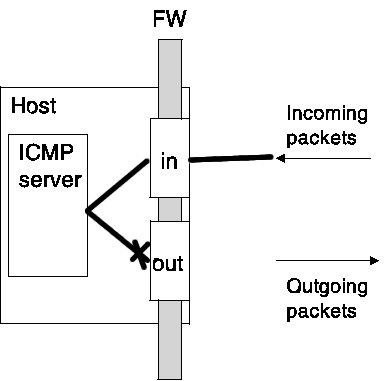
\includegraphics[scale=0.5]{figures/icmpexample-out}
           \label{fig:icmpexampleQ1}
        }
        \hspace{1in}
        \subfigure[Use this Figure to explain Q2]{
           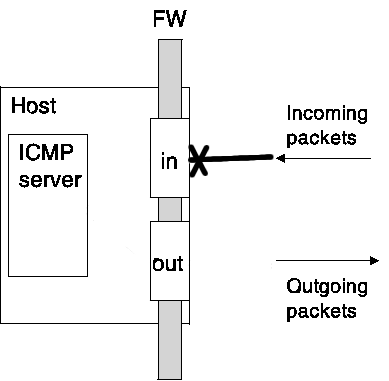
\includegraphics[scale=0.5]{figures/icmpexample-in}
           \label{fig:icmpexampleQ2}
        }
    \end{center}
    \caption{Figure to help you illustrate your thoughts regarding the packet 
        flow in questions Q1 and Q2.}
    \label{fig:icmpexample}
\end{figure}


\noindent \textbf{Q3. For each entry in the log, several information items are
displayed. Some entries can be useful for creating new rules. Explain the 
items {\texttt IN}, {\texttt OUT}, {\texttt SRC}, {\texttt DST} and {\texttt PROTO}
mean and why these might be useful.}
 
Not applicable. The logging did not work for anyone during the lab. File permissions?
\\

\noindent \textbf{Q4. At this stage, with default policy set to DROP for all 
chains, would you consider the system secure? Would you consider it useful?}

The system is most certainly secure but not usefull. If no traffic att all will
be let through the only security holes would be if there is any implementation 
bugs in the firwall. Other attacks like DoS will allso work. 
\\

\noindent \textbf{Q5. Assume instead that you used default policy ACCEPT, 
would you consider the system secure now? Would you consider it useful?}

With a policy of ACCEPT and no other rules everything will work without interference
from the firewall. This would be the same as turning the firewall off. If you add
the appropriate rules the system could be made just as secure as with policy DROP but
this aproach is much more prone to human error.
\\

\noindent \textbf{Q6. You just added some protection against flooding by 
limiting the number of packets the firewall will let through to 1 per second. 
Give two examples on how you can tell that you are protected!}

By sending a ping storm from another host and se that our host only responds to 1 per 
second. We can also use wireshark on the host an see that the host only handles 1 
ping per second.


\end{document}
